\documentclass[twoside]{book}

% Packages required by doxygen
\usepackage{fixltx2e}
\usepackage{calc}
\usepackage{doxygen}
\usepackage[export]{adjustbox} % also loads graphicx
\usepackage{graphicx}
\usepackage[utf8]{inputenc}
\usepackage{makeidx}
\usepackage{multicol}
\usepackage{multirow}
\PassOptionsToPackage{warn}{textcomp}
\usepackage{textcomp}
\usepackage[nointegrals]{wasysym}
\usepackage[table]{xcolor}

% Font selection
\usepackage[T1]{fontenc}
\usepackage[scaled=.90]{helvet}
\usepackage{courier}
\usepackage{amssymb}
\usepackage{sectsty}
\renewcommand{\familydefault}{\sfdefault}
\allsectionsfont{%
  \fontseries{bc}\selectfont%
  \color{darkgray}%
}
\renewcommand{\DoxyLabelFont}{%
  \fontseries{bc}\selectfont%
  \color{darkgray}%
}
\newcommand{\+}{\discretionary{\mbox{\scriptsize$\hookleftarrow$}}{}{}}

% Page & text layout
\usepackage{geometry}
\geometry{%
  a4paper,%
  top=2.5cm,%
  bottom=2.5cm,%
  left=2.5cm,%
  right=2.5cm%
}
\tolerance=750
\hfuzz=15pt
\hbadness=750
\setlength{\emergencystretch}{15pt}
\setlength{\parindent}{0cm}
\setlength{\parskip}{0.2cm}
\makeatletter
\renewcommand{\paragraph}{%
  \@startsection{paragraph}{4}{0ex}{-1.0ex}{1.0ex}{%
    \normalfont\normalsize\bfseries\SS@parafont%
  }%
}
\renewcommand{\subparagraph}{%
  \@startsection{subparagraph}{5}{0ex}{-1.0ex}{1.0ex}{%
    \normalfont\normalsize\bfseries\SS@subparafont%
  }%
}
\makeatother

% Headers & footers
\usepackage{fancyhdr}
\pagestyle{fancyplain}
\fancyhead[LE]{\fancyplain{}{\bfseries\thepage}}
\fancyhead[CE]{\fancyplain{}{}}
\fancyhead[RE]{\fancyplain{}{\bfseries\leftmark}}
\fancyhead[LO]{\fancyplain{}{\bfseries\rightmark}}
\fancyhead[CO]{\fancyplain{}{}}
\fancyhead[RO]{\fancyplain{}{\bfseries\thepage}}
\fancyfoot[LE]{\fancyplain{}{}}
\fancyfoot[CE]{\fancyplain{}{}}
\fancyfoot[RE]{\fancyplain{}{\bfseries\scriptsize Generated on Fri Oct 14 2016 13\+:15\+:22 for Dynet by Doxygen }}
\fancyfoot[LO]{\fancyplain{}{\bfseries\scriptsize Generated on Fri Oct 14 2016 13\+:15\+:22 for Dynet by Doxygen }}
\fancyfoot[CO]{\fancyplain{}{}}
\fancyfoot[RO]{\fancyplain{}{}}
\renewcommand{\footrulewidth}{0.4pt}
\renewcommand{\chaptermark}[1]{%
  \markboth{#1}{}%
}
\renewcommand{\sectionmark}[1]{%
  \markright{\thesection\ #1}%
}

% Indices & bibliography
\usepackage{natbib}
\usepackage[titles]{tocloft}
\setcounter{tocdepth}{3}
\setcounter{secnumdepth}{5}
\makeindex

% Hyperlinks (required, but should be loaded last)
\usepackage{ifpdf}
\ifpdf
  \usepackage[pdftex,pagebackref=true]{hyperref}
\else
  \usepackage[ps2pdf,pagebackref=true]{hyperref}
\fi
\hypersetup{%
  colorlinks=true,%
  linkcolor=blue,%
  citecolor=blue,%
  unicode%
}

% Custom commands
\newcommand{\clearemptydoublepage}{%
  \newpage{\pagestyle{empty}\cleardoublepage}%
}


%===== C O N T E N T S =====

\begin{document}

% Titlepage & ToC
\hypersetup{pageanchor=false,
             bookmarks=true,
             bookmarksnumbered=true,
             pdfencoding=unicode
            }
\pagenumbering{roman}
\begin{titlepage}
\vspace*{7cm}
\begin{center}%
{\Large Dynet }\\
\vspace*{1cm}
{\large Generated by Doxygen 1.8.9.1}\\
\vspace*{0.5cm}
{\small Fri Oct 14 2016 13:15:22}\\
\end{center}
\end{titlepage}
\clearemptydoublepage
\tableofcontents
\clearemptydoublepage
\pagenumbering{arabic}
\hypersetup{pageanchor=true}

%--- Begin generated contents ---
\chapter{Hierarchical Index}
\section{Class Hierarchy}
This inheritance list is sorted roughly, but not completely, alphabetically\+:\begin{DoxyCompactList}
\item \contentsline{section}{dynet\+:\+:expr\+:\+:Expression}{\pageref{structdynet_1_1expr_1_1Expression}}{}
\item \contentsline{section}{dynet\+:\+:Trainer}{\pageref{structdynet_1_1Trainer}}{}
\begin{DoxyCompactList}
\item \contentsline{section}{dynet\+:\+:Adadelta\+Trainer}{\pageref{structdynet_1_1AdadeltaTrainer}}{}
\item \contentsline{section}{dynet\+:\+:Adagrad\+Trainer}{\pageref{structdynet_1_1AdagradTrainer}}{}
\item \contentsline{section}{dynet\+:\+:Adam\+Trainer}{\pageref{structdynet_1_1AdamTrainer}}{}
\item \contentsline{section}{dynet\+:\+:Momentum\+S\+G\+D\+Trainer}{\pageref{structdynet_1_1MomentumSGDTrainer}}{}
\item \contentsline{section}{dynet\+:\+:Rms\+Prop\+Trainer}{\pageref{structdynet_1_1RmsPropTrainer}}{}
\item \contentsline{section}{dynet\+:\+:Simple\+S\+G\+D\+Trainer}{\pageref{structdynet_1_1SimpleSGDTrainer}}{}
\end{DoxyCompactList}
\end{DoxyCompactList}

\chapter{Class Index}
\section{Class List}
Here are the classes, structs, unions and interfaces with brief descriptions\+:\begin{DoxyCompactList}
\item\contentsline{section}{\hyperlink{structdynet_1_1AdadeltaTrainer}{dynet\+::\+Adadelta\+Trainer} }{\pageref{structdynet_1_1AdadeltaTrainer}}{}
\item\contentsline{section}{\hyperlink{structdynet_1_1AdagradTrainer}{dynet\+::\+Adagrad\+Trainer} }{\pageref{structdynet_1_1AdagradTrainer}}{}
\item\contentsline{section}{\hyperlink{structdynet_1_1AdamTrainer}{dynet\+::\+Adam\+Trainer} }{\pageref{structdynet_1_1AdamTrainer}}{}
\item\contentsline{section}{\hyperlink{structdynet_1_1expr_1_1Expression}{dynet\+::expr\+::\+Expression} }{\pageref{structdynet_1_1expr_1_1Expression}}{}
\item\contentsline{section}{\hyperlink{structdynet_1_1MomentumSGDTrainer}{dynet\+::\+Momentum\+S\+G\+D\+Trainer} }{\pageref{structdynet_1_1MomentumSGDTrainer}}{}
\item\contentsline{section}{\hyperlink{structdynet_1_1RmsPropTrainer}{dynet\+::\+Rms\+Prop\+Trainer} }{\pageref{structdynet_1_1RmsPropTrainer}}{}
\item\contentsline{section}{\hyperlink{structdynet_1_1SimpleSGDTrainer}{dynet\+::\+Simple\+S\+G\+D\+Trainer} }{\pageref{structdynet_1_1SimpleSGDTrainer}}{}
\item\contentsline{section}{\hyperlink{structdynet_1_1Trainer}{dynet\+::\+Trainer} }{\pageref{structdynet_1_1Trainer}}{}
\end{DoxyCompactList}

\chapter{Class Documentation}
\hypertarget{structdynet_1_1AdadeltaTrainer}{}\section{dynet\+:\+:Adadelta\+Trainer Struct Reference}
\label{structdynet_1_1AdadeltaTrainer}\index{dynet\+::\+Adadelta\+Trainer@{dynet\+::\+Adadelta\+Trainer}}


Inheritance diagram for dynet\+:\+:Adadelta\+Trainer\+:\nopagebreak
\begin{figure}[H]
\begin{center}
\leavevmode
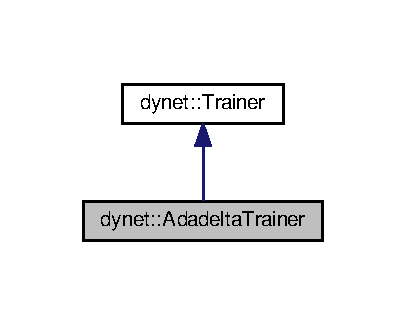
\includegraphics[width=195pt]{structdynet_1_1AdadeltaTrainer__inherit__graph}
\end{center}
\end{figure}


Collaboration diagram for dynet\+:\+:Adadelta\+Trainer\+:\nopagebreak
\begin{figure}[H]
\begin{center}
\leavevmode
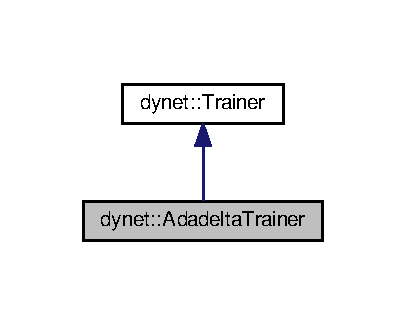
\includegraphics[width=195pt]{structdynet_1_1AdadeltaTrainer__coll__graph}
\end{center}
\end{figure}
\subsection*{Public Member Functions}
\begin{DoxyCompactItemize}
\item 
\hypertarget{structdynet_1_1AdadeltaTrainer_aaed979b129d3a4642321b8d414efea0c}{}{\bfseries Adadelta\+Trainer} (Model $\ast$m, real eps=1e-\/6, real rho=0.\+95)\label{structdynet_1_1AdadeltaTrainer_aaed979b129d3a4642321b8d414efea0c}

\end{DoxyCompactItemize}
\subsection*{Protected Member Functions}
\begin{DoxyCompactItemize}
\item 
\hypertarget{structdynet_1_1AdadeltaTrainer_a98d5d3abe044d455df1a0fb3c35fbf44}{}virtual void {\bfseries alloc\+\_\+impl} () override\label{structdynet_1_1AdadeltaTrainer_a98d5d3abe044d455df1a0fb3c35fbf44}

\end{DoxyCompactItemize}
\subsection*{Protected Attributes}
\begin{DoxyCompactItemize}
\item 
\hypertarget{structdynet_1_1AdadeltaTrainer_a65675903e5b9d77c7adde456d85d7b8c}{}real {\bfseries epsilon}\label{structdynet_1_1AdadeltaTrainer_a65675903e5b9d77c7adde456d85d7b8c}

\item 
\hypertarget{structdynet_1_1AdadeltaTrainer_a41208d6c68aa6478a661aac929b335e6}{}real {\bfseries rho}\label{structdynet_1_1AdadeltaTrainer_a41208d6c68aa6478a661aac929b335e6}

\item 
\hypertarget{structdynet_1_1AdadeltaTrainer_a51fb513277530881e6cbe16222adfff8}{}std\+::vector$<$ Shadow\+Parameters $>$ {\bfseries hg}\label{structdynet_1_1AdadeltaTrainer_a51fb513277530881e6cbe16222adfff8}

\item 
\hypertarget{structdynet_1_1AdadeltaTrainer_a3150eb1db93079ca53e470265c0a81df}{}std\+::vector$<$ Shadow\+Lookup\+Parameters $>$ {\bfseries hlg}\label{structdynet_1_1AdadeltaTrainer_a3150eb1db93079ca53e470265c0a81df}

\item 
\hypertarget{structdynet_1_1AdadeltaTrainer_a835052dcc3f77e01016afb8de0a9c4b0}{}std\+::vector$<$ Shadow\+Parameters $>$ {\bfseries hd}\label{structdynet_1_1AdadeltaTrainer_a835052dcc3f77e01016afb8de0a9c4b0}

\item 
\hypertarget{structdynet_1_1AdadeltaTrainer_a1dbae7cb54caba3e863f5a7c97934fe6}{}std\+::vector$<$ Shadow\+Lookup\+Parameters $>$ {\bfseries hld}\label{structdynet_1_1AdadeltaTrainer_a1dbae7cb54caba3e863f5a7c97934fe6}

\end{DoxyCompactItemize}
\subsection*{Friends}
\begin{DoxyCompactItemize}
\item 
\hypertarget{structdynet_1_1AdadeltaTrainer_ac98d07dd8f7b70e16ccb9a01abf56b9c}{}class {\bfseries boost\+::serialization\+::access}\label{structdynet_1_1AdadeltaTrainer_ac98d07dd8f7b70e16ccb9a01abf56b9c}

\end{DoxyCompactItemize}
\subsection*{Additional Inherited Members}


The documentation for this struct was generated from the following file\+:\begin{DoxyCompactItemize}
\item 
/home/paul/dev/dynet/dynet/training.\+h\end{DoxyCompactItemize}

\hypertarget{structdynet_1_1AdagradTrainer}{}\section{dynet\+:\+:Adagrad\+Trainer Struct Reference}
\label{structdynet_1_1AdagradTrainer}\index{dynet\+::\+Adagrad\+Trainer@{dynet\+::\+Adagrad\+Trainer}}


Inheritance diagram for dynet\+:\+:Adagrad\+Trainer\+:\nopagebreak
\begin{figure}[H]
\begin{center}
\leavevmode
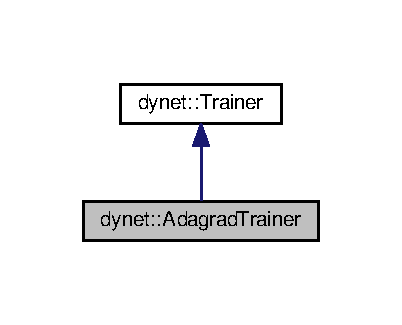
\includegraphics[width=193pt]{structdynet_1_1AdagradTrainer__inherit__graph}
\end{center}
\end{figure}


Collaboration diagram for dynet\+:\+:Adagrad\+Trainer\+:\nopagebreak
\begin{figure}[H]
\begin{center}
\leavevmode
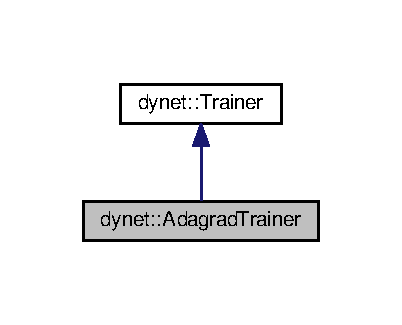
\includegraphics[width=193pt]{structdynet_1_1AdagradTrainer__coll__graph}
\end{center}
\end{figure}
\subsection*{Public Member Functions}
\begin{DoxyCompactItemize}
\item 
\hypertarget{structdynet_1_1AdagradTrainer_a5e4c3a6215a907fe324b91d44be79f65}{}{\bfseries Adagrad\+Trainer} (Model $\ast$m, real e0=0.\+1, real eps=1e-\/20)\label{structdynet_1_1AdagradTrainer_a5e4c3a6215a907fe324b91d44be79f65}

\end{DoxyCompactItemize}
\subsection*{Protected Member Functions}
\begin{DoxyCompactItemize}
\item 
\hypertarget{structdynet_1_1AdagradTrainer_a59aedeee8ebf2381aae2e621dc0933ba}{}virtual void {\bfseries alloc\+\_\+impl} () override\label{structdynet_1_1AdagradTrainer_a59aedeee8ebf2381aae2e621dc0933ba}

\end{DoxyCompactItemize}
\subsection*{Protected Attributes}
\begin{DoxyCompactItemize}
\item 
\hypertarget{structdynet_1_1AdagradTrainer_aec2c7f16d917701afcc033e74df521ce}{}real {\bfseries epsilon}\label{structdynet_1_1AdagradTrainer_aec2c7f16d917701afcc033e74df521ce}

\item 
\hypertarget{structdynet_1_1AdagradTrainer_acec2f473f86ca026818ae76c8b3172cc}{}std\+::vector$<$ Shadow\+Parameters $>$ {\bfseries vp}\label{structdynet_1_1AdagradTrainer_acec2f473f86ca026818ae76c8b3172cc}

\item 
\hypertarget{structdynet_1_1AdagradTrainer_a4198955558c37a432400f163aada58f6}{}std\+::vector$<$ Shadow\+Lookup\+Parameters $>$ {\bfseries vlp}\label{structdynet_1_1AdagradTrainer_a4198955558c37a432400f163aada58f6}

\end{DoxyCompactItemize}
\subsection*{Friends}
\begin{DoxyCompactItemize}
\item 
\hypertarget{structdynet_1_1AdagradTrainer_ac98d07dd8f7b70e16ccb9a01abf56b9c}{}class {\bfseries boost\+::serialization\+::access}\label{structdynet_1_1AdagradTrainer_ac98d07dd8f7b70e16ccb9a01abf56b9c}

\end{DoxyCompactItemize}
\subsection*{Additional Inherited Members}


The documentation for this struct was generated from the following file\+:\begin{DoxyCompactItemize}
\item 
/home/paul/dev/dynet/dynet/training.\+h\end{DoxyCompactItemize}

\hypertarget{structdynet_1_1AdamTrainer}{}\section{dynet\+:\+:Adam\+Trainer Struct Reference}
\label{structdynet_1_1AdamTrainer}\index{dynet\+::\+Adam\+Trainer@{dynet\+::\+Adam\+Trainer}}


Inheritance diagram for dynet\+:\+:Adam\+Trainer\+:\nopagebreak
\begin{figure}[H]
\begin{center}
\leavevmode
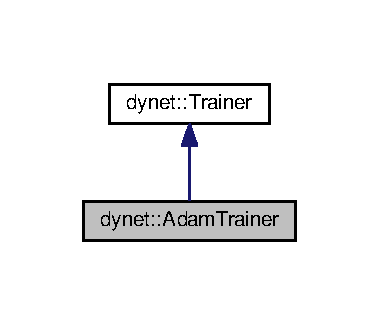
\includegraphics[width=182pt]{structdynet_1_1AdamTrainer__inherit__graph}
\end{center}
\end{figure}


Collaboration diagram for dynet\+:\+:Adam\+Trainer\+:\nopagebreak
\begin{figure}[H]
\begin{center}
\leavevmode
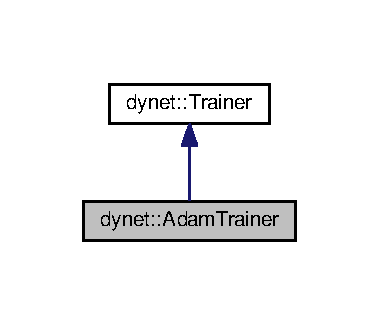
\includegraphics[width=182pt]{structdynet_1_1AdamTrainer__coll__graph}
\end{center}
\end{figure}
\subsection*{Public Member Functions}
\begin{DoxyCompactItemize}
\item 
\hypertarget{structdynet_1_1AdamTrainer_a4990f1adf7d703209f12333cd6956642}{}{\bfseries Adam\+Trainer} (Model $\ast$m, float alpha=0.\+001, float beta\+\_\+1=0.\+9, float beta\+\_\+2=0.\+999, float eps=1e-\/8)\label{structdynet_1_1AdamTrainer_a4990f1adf7d703209f12333cd6956642}

\end{DoxyCompactItemize}
\subsection*{Protected Member Functions}
\begin{DoxyCompactItemize}
\item 
\hypertarget{structdynet_1_1AdamTrainer_a17f07f2cfcbd03641a12475b2c739a7c}{}virtual void {\bfseries alloc\+\_\+impl} () override\label{structdynet_1_1AdamTrainer_a17f07f2cfcbd03641a12475b2c739a7c}

\end{DoxyCompactItemize}
\subsection*{Protected Attributes}
\begin{DoxyCompactItemize}
\item 
\hypertarget{structdynet_1_1AdamTrainer_aae8746433c7394dddc78849e49402f1f}{}float {\bfseries beta\+\_\+1}\label{structdynet_1_1AdamTrainer_aae8746433c7394dddc78849e49402f1f}

\item 
\hypertarget{structdynet_1_1AdamTrainer_a6089112f88ea42b5c178a3e71b405734}{}float {\bfseries beta\+\_\+2}\label{structdynet_1_1AdamTrainer_a6089112f88ea42b5c178a3e71b405734}

\item 
\hypertarget{structdynet_1_1AdamTrainer_a125ca67ff4ce57e896950102b26679cf}{}float {\bfseries epsilon}\label{structdynet_1_1AdamTrainer_a125ca67ff4ce57e896950102b26679cf}

\item 
\hypertarget{structdynet_1_1AdamTrainer_abae9d7b1df4a4bf4d849dbd2ededc2c8}{}std\+::vector$<$ Shadow\+Parameters $>$ {\bfseries m}\label{structdynet_1_1AdamTrainer_abae9d7b1df4a4bf4d849dbd2ededc2c8}

\item 
\hypertarget{structdynet_1_1AdamTrainer_a36fee69c4827e4a1de6fbcde35977305}{}std\+::vector$<$ Shadow\+Lookup\+Parameters $>$ {\bfseries lm}\label{structdynet_1_1AdamTrainer_a36fee69c4827e4a1de6fbcde35977305}

\item 
\hypertarget{structdynet_1_1AdamTrainer_a3e0f0cfdf210edd1c6e7c258bf5f480c}{}std\+::vector$<$ Shadow\+Parameters $>$ {\bfseries v}\label{structdynet_1_1AdamTrainer_a3e0f0cfdf210edd1c6e7c258bf5f480c}

\item 
\hypertarget{structdynet_1_1AdamTrainer_a641513dd5cba85c96e35a275ecf3f2b5}{}std\+::vector$<$ Shadow\+Lookup\+Parameters $>$ {\bfseries lv}\label{structdynet_1_1AdamTrainer_a641513dd5cba85c96e35a275ecf3f2b5}

\end{DoxyCompactItemize}
\subsection*{Friends}
\begin{DoxyCompactItemize}
\item 
\hypertarget{structdynet_1_1AdamTrainer_ac98d07dd8f7b70e16ccb9a01abf56b9c}{}class {\bfseries boost\+::serialization\+::access}\label{structdynet_1_1AdamTrainer_ac98d07dd8f7b70e16ccb9a01abf56b9c}

\end{DoxyCompactItemize}
\subsection*{Additional Inherited Members}


The documentation for this struct was generated from the following file\+:\begin{DoxyCompactItemize}
\item 
/home/paul/dev/dynet/dynet/training.\+h\end{DoxyCompactItemize}

\hypertarget{structdynet_1_1expr_1_1Expression}{}\section{dynet\+:\+:expr\+:\+:Expression Struct Reference}
\label{structdynet_1_1expr_1_1Expression}\index{dynet\+::expr\+::\+Expression@{dynet\+::expr\+::\+Expression}}
\subsection*{Public Member Functions}
\begin{DoxyCompactItemize}
\item 
\hypertarget{structdynet_1_1expr_1_1Expression_a2bf2dd30fa0fdf2956090cd39f5b52dc}{}{\bfseries Expression} (Computation\+Graph $\ast$pg, Variable\+Index i)\label{structdynet_1_1expr_1_1Expression_a2bf2dd30fa0fdf2956090cd39f5b52dc}

\item 
\hypertarget{structdynet_1_1expr_1_1Expression_a34dfa51f88f52de548e219a458e81731}{}const Tensor \& {\bfseries value} () const \label{structdynet_1_1expr_1_1Expression_a34dfa51f88f52de548e219a458e81731}

\end{DoxyCompactItemize}
\subsection*{Public Attributes}
\begin{DoxyCompactItemize}
\item 
\hypertarget{structdynet_1_1expr_1_1Expression_a59221401f07f495340c5f6a5a29dadf5}{}Computation\+Graph $\ast$ {\bfseries pg}\label{structdynet_1_1expr_1_1Expression_a59221401f07f495340c5f6a5a29dadf5}

\item 
\hypertarget{structdynet_1_1expr_1_1Expression_a3d108e0edb73b2d38789a3a6a2dd5434}{}Variable\+Index {\bfseries i}\label{structdynet_1_1expr_1_1Expression_a3d108e0edb73b2d38789a3a6a2dd5434}

\end{DoxyCompactItemize}


The documentation for this struct was generated from the following file\+:\begin{DoxyCompactItemize}
\item 
/home/paul/dev/dynet/dynet/expr.\+h\end{DoxyCompactItemize}

\hypertarget{structdynet_1_1MomentumSGDTrainer}{}\section{dynet\+:\+:Momentum\+S\+G\+D\+Trainer Struct Reference}
\label{structdynet_1_1MomentumSGDTrainer}\index{dynet\+::\+Momentum\+S\+G\+D\+Trainer@{dynet\+::\+Momentum\+S\+G\+D\+Trainer}}


Inheritance diagram for dynet\+:\+:Momentum\+S\+G\+D\+Trainer\+:\nopagebreak
\begin{figure}[H]
\begin{center}
\leavevmode
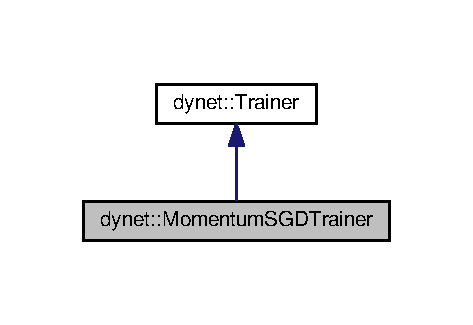
\includegraphics[width=227pt]{structdynet_1_1MomentumSGDTrainer__inherit__graph}
\end{center}
\end{figure}


Collaboration diagram for dynet\+:\+:Momentum\+S\+G\+D\+Trainer\+:\nopagebreak
\begin{figure}[H]
\begin{center}
\leavevmode
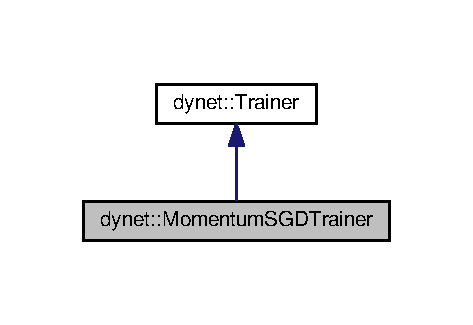
\includegraphics[width=227pt]{structdynet_1_1MomentumSGDTrainer__coll__graph}
\end{center}
\end{figure}
\subsection*{Public Member Functions}
\begin{DoxyCompactItemize}
\item 
\hypertarget{structdynet_1_1MomentumSGDTrainer_a29ba25e1ad153bc552edc178a69c67c7}{}{\bfseries Momentum\+S\+G\+D\+Trainer} (Model $\ast$m, real e0=0.\+01, real mom=0.\+9)\label{structdynet_1_1MomentumSGDTrainer_a29ba25e1ad153bc552edc178a69c67c7}

\end{DoxyCompactItemize}
\subsection*{Protected Member Functions}
\begin{DoxyCompactItemize}
\item 
\hypertarget{structdynet_1_1MomentumSGDTrainer_a904d0442ffa5d18463ca529ee07a1af2}{}virtual void {\bfseries alloc\+\_\+impl} () override\label{structdynet_1_1MomentumSGDTrainer_a904d0442ffa5d18463ca529ee07a1af2}

\end{DoxyCompactItemize}
\subsection*{Protected Attributes}
\begin{DoxyCompactItemize}
\item 
\hypertarget{structdynet_1_1MomentumSGDTrainer_a61b272617d6a7a80f13f4c8d03215a7b}{}real {\bfseries momentum}\label{structdynet_1_1MomentumSGDTrainer_a61b272617d6a7a80f13f4c8d03215a7b}

\item 
\hypertarget{structdynet_1_1MomentumSGDTrainer_af6d25b4fbf842543c8de00470bfa0cbc}{}std\+::vector$<$ Shadow\+Parameters $>$ {\bfseries vp}\label{structdynet_1_1MomentumSGDTrainer_af6d25b4fbf842543c8de00470bfa0cbc}

\item 
\hypertarget{structdynet_1_1MomentumSGDTrainer_aea8235a50ab0e66768bd453e01cb406a}{}std\+::vector$<$ Shadow\+Lookup\+Parameters $>$ {\bfseries vlp}\label{structdynet_1_1MomentumSGDTrainer_aea8235a50ab0e66768bd453e01cb406a}

\end{DoxyCompactItemize}
\subsection*{Friends}
\begin{DoxyCompactItemize}
\item 
\hypertarget{structdynet_1_1MomentumSGDTrainer_ac98d07dd8f7b70e16ccb9a01abf56b9c}{}class {\bfseries boost\+::serialization\+::access}\label{structdynet_1_1MomentumSGDTrainer_ac98d07dd8f7b70e16ccb9a01abf56b9c}

\end{DoxyCompactItemize}
\subsection*{Additional Inherited Members}


The documentation for this struct was generated from the following file\+:\begin{DoxyCompactItemize}
\item 
/home/paul/dev/dynet/dynet/training.\+h\end{DoxyCompactItemize}

\hypertarget{structdynet_1_1RmsPropTrainer}{}\section{dynet\+:\+:Rms\+Prop\+Trainer Struct Reference}
\label{structdynet_1_1RmsPropTrainer}\index{dynet\+::\+Rms\+Prop\+Trainer@{dynet\+::\+Rms\+Prop\+Trainer}}


Inheritance diagram for dynet\+:\+:Rms\+Prop\+Trainer\+:\nopagebreak
\begin{figure}[H]
\begin{center}
\leavevmode
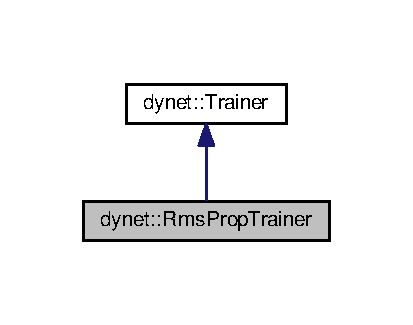
\includegraphics[width=198pt]{structdynet_1_1RmsPropTrainer__inherit__graph}
\end{center}
\end{figure}


Collaboration diagram for dynet\+:\+:Rms\+Prop\+Trainer\+:\nopagebreak
\begin{figure}[H]
\begin{center}
\leavevmode
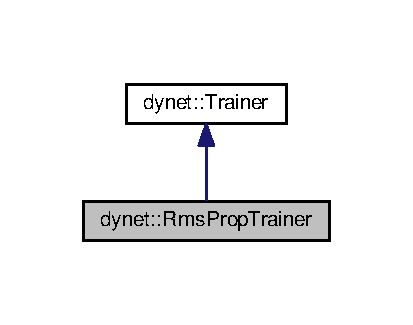
\includegraphics[width=198pt]{structdynet_1_1RmsPropTrainer__coll__graph}
\end{center}
\end{figure}
\subsection*{Public Member Functions}
\begin{DoxyCompactItemize}
\item 
\hypertarget{structdynet_1_1RmsPropTrainer_a80f7706c329f61f0a0f828f9795471e5}{}{\bfseries Rms\+Prop\+Trainer} (Model $\ast$m, real e0=0.\+1, real eps=1e-\/20, real rho=0.\+95)\label{structdynet_1_1RmsPropTrainer_a80f7706c329f61f0a0f828f9795471e5}

\end{DoxyCompactItemize}
\subsection*{Protected Member Functions}
\begin{DoxyCompactItemize}
\item 
\hypertarget{structdynet_1_1RmsPropTrainer_a7161b50fbf7673c7c7c7180c1e591e81}{}virtual void {\bfseries alloc\+\_\+impl} () override\label{structdynet_1_1RmsPropTrainer_a7161b50fbf7673c7c7c7180c1e591e81}

\end{DoxyCompactItemize}
\subsection*{Protected Attributes}
\begin{DoxyCompactItemize}
\item 
\hypertarget{structdynet_1_1RmsPropTrainer_abea2f280bd81e66c84d19243240e5d07}{}real {\bfseries epsilon}\label{structdynet_1_1RmsPropTrainer_abea2f280bd81e66c84d19243240e5d07}

\item 
\hypertarget{structdynet_1_1RmsPropTrainer_aa32e89c3dd7251f0315d05e09376f97f}{}real {\bfseries rho}\label{structdynet_1_1RmsPropTrainer_aa32e89c3dd7251f0315d05e09376f97f}

\item 
\hypertarget{structdynet_1_1RmsPropTrainer_af700a2a0cc9dc136a98a7260522c5947}{}std\+::vector$<$ real $>$ {\bfseries hg}\label{structdynet_1_1RmsPropTrainer_af700a2a0cc9dc136a98a7260522c5947}

\item 
\hypertarget{structdynet_1_1RmsPropTrainer_aef4e1f6d56c30ef3d5d1d01d2b2df918}{}std\+::vector$<$ std\+::vector$<$ real $>$ $>$ {\bfseries hlg}\label{structdynet_1_1RmsPropTrainer_aef4e1f6d56c30ef3d5d1d01d2b2df918}

\end{DoxyCompactItemize}
\subsection*{Friends}
\begin{DoxyCompactItemize}
\item 
\hypertarget{structdynet_1_1RmsPropTrainer_ac98d07dd8f7b70e16ccb9a01abf56b9c}{}class {\bfseries boost\+::serialization\+::access}\label{structdynet_1_1RmsPropTrainer_ac98d07dd8f7b70e16ccb9a01abf56b9c}

\end{DoxyCompactItemize}
\subsection*{Additional Inherited Members}


The documentation for this struct was generated from the following file\+:\begin{DoxyCompactItemize}
\item 
/home/paul/dev/dynet/dynet/training.\+h\end{DoxyCompactItemize}

\hypertarget{structdynet_1_1SimpleSGDTrainer}{}\section{dynet\+:\+:Simple\+S\+G\+D\+Trainer Struct Reference}
\label{structdynet_1_1SimpleSGDTrainer}\index{dynet\+::\+Simple\+S\+G\+D\+Trainer@{dynet\+::\+Simple\+S\+G\+D\+Trainer}}


Inheritance diagram for dynet\+:\+:Simple\+S\+G\+D\+Trainer\+:\nopagebreak
\begin{figure}[H]
\begin{center}
\leavevmode
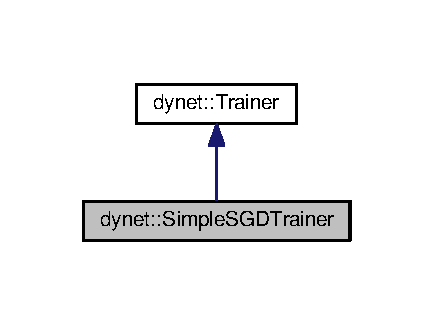
\includegraphics[width=208pt]{structdynet_1_1SimpleSGDTrainer__inherit__graph}
\end{center}
\end{figure}


Collaboration diagram for dynet\+:\+:Simple\+S\+G\+D\+Trainer\+:\nopagebreak
\begin{figure}[H]
\begin{center}
\leavevmode
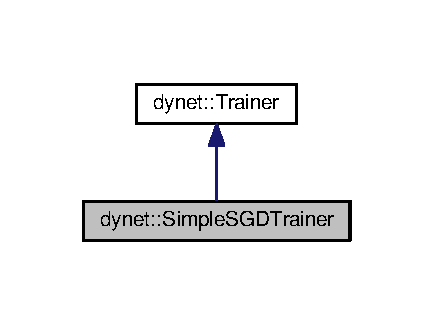
\includegraphics[width=208pt]{structdynet_1_1SimpleSGDTrainer__coll__graph}
\end{center}
\end{figure}
\subsection*{Public Member Functions}
\begin{DoxyCompactItemize}
\item 
\hypertarget{structdynet_1_1SimpleSGDTrainer_ac3d5dd3f59db29f7d803130f874f9832}{}{\bfseries Simple\+S\+G\+D\+Trainer} (Model $\ast$m, real e0=0.\+1)\label{structdynet_1_1SimpleSGDTrainer_ac3d5dd3f59db29f7d803130f874f9832}

\end{DoxyCompactItemize}
\subsection*{Friends}
\begin{DoxyCompactItemize}
\item 
\hypertarget{structdynet_1_1SimpleSGDTrainer_ac98d07dd8f7b70e16ccb9a01abf56b9c}{}class {\bfseries boost\+::serialization\+::access}\label{structdynet_1_1SimpleSGDTrainer_ac98d07dd8f7b70e16ccb9a01abf56b9c}

\end{DoxyCompactItemize}
\subsection*{Additional Inherited Members}


The documentation for this struct was generated from the following file\+:\begin{DoxyCompactItemize}
\item 
/home/paul/dev/dynet/dynet/training.\+h\end{DoxyCompactItemize}

\hypertarget{structdynet_1_1Trainer}{}\section{dynet\+:\+:Trainer Struct Reference}
\label{structdynet_1_1Trainer}\index{dynet\+::\+Trainer@{dynet\+::\+Trainer}}


Inheritance diagram for dynet\+:\+:Trainer\+:\nopagebreak
\begin{figure}[H]
\begin{center}
\leavevmode
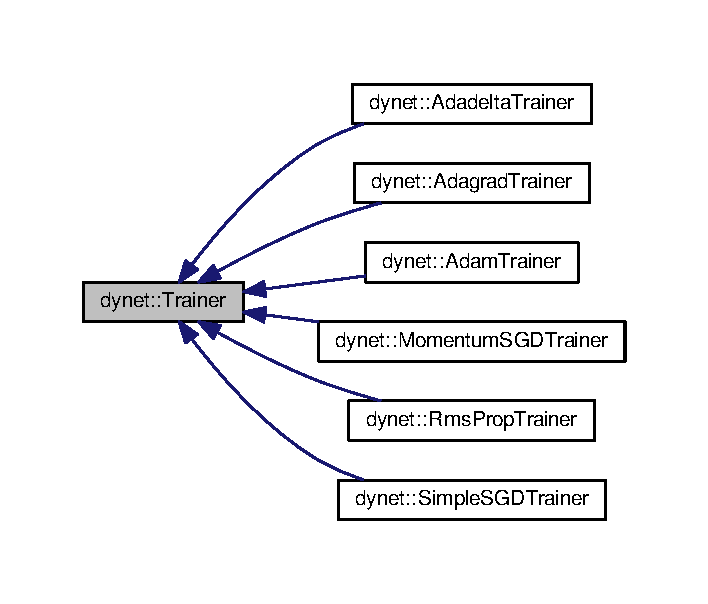
\includegraphics[width=340pt]{structdynet_1_1Trainer__inherit__graph}
\end{center}
\end{figure}
\subsection*{Public Member Functions}
\begin{DoxyCompactItemize}
\item 
\hypertarget{structdynet_1_1Trainer_aebf069a0e0f27965d3e2c83ee2634fac}{}{\bfseries Trainer} (Model $\ast$m, real e0)\label{structdynet_1_1Trainer_aebf069a0e0f27965d3e2c83ee2634fac}

\item 
\hypertarget{structdynet_1_1Trainer_aeef0722fc13d630e11bb0eb87c1c0022}{}void {\bfseries update} (real scale=1.\+0)\label{structdynet_1_1Trainer_aeef0722fc13d630e11bb0eb87c1c0022}

\item 
\hypertarget{structdynet_1_1Trainer_a2e3ea5a9d5b7ef3b5e6d369b3c5e27b9}{}void {\bfseries update\+\_\+epoch} (real r=1)\label{structdynet_1_1Trainer_a2e3ea5a9d5b7ef3b5e6d369b3c5e27b9}

\item 
\hypertarget{structdynet_1_1Trainer_aded3359afcae9dcea200fc41efe4de05}{}float {\bfseries clip\+\_\+gradients} ()\label{structdynet_1_1Trainer_aded3359afcae9dcea200fc41efe4de05}

\item 
\hypertarget{structdynet_1_1Trainer_a1cf3844683089def105240184f1c4fbc}{}void {\bfseries rescale\+\_\+and\+\_\+reset\+\_\+weight\+\_\+decay} ()\label{structdynet_1_1Trainer_a1cf3844683089def105240184f1c4fbc}

\item 
\hypertarget{structdynet_1_1Trainer_a705582c0d3e884e1f4b35704ec03bb08}{}void {\bfseries status} ()\label{structdynet_1_1Trainer_a705582c0d3e884e1f4b35704ec03bb08}

\end{DoxyCompactItemize}
\subsection*{Public Attributes}
\begin{DoxyCompactItemize}
\item 
\hypertarget{structdynet_1_1Trainer_a6b3c3ffe009d23b2ffc38eef19081c33}{}real {\bfseries eta0}\label{structdynet_1_1Trainer_a6b3c3ffe009d23b2ffc38eef19081c33}

\item 
\hypertarget{structdynet_1_1Trainer_ad4d96038e7fdd4bbf92e977482185183}{}real {\bfseries eta}\label{structdynet_1_1Trainer_ad4d96038e7fdd4bbf92e977482185183}

\item 
\hypertarget{structdynet_1_1Trainer_a87fb458762795170c09689aa8f9e7d35}{}real {\bfseries eta\+\_\+decay}\label{structdynet_1_1Trainer_a87fb458762795170c09689aa8f9e7d35}

\item 
\hypertarget{structdynet_1_1Trainer_a34f348c0027687a2ab74d32b489c47df}{}real {\bfseries epoch}\label{structdynet_1_1Trainer_a34f348c0027687a2ab74d32b489c47df}

\item 
\hypertarget{structdynet_1_1Trainer_ab34bfbb2aaa719d9d7829c5b679a141b}{}real {\bfseries clipping\+\_\+enabled}\label{structdynet_1_1Trainer_ab34bfbb2aaa719d9d7829c5b679a141b}

\item 
\hypertarget{structdynet_1_1Trainer_a5dceed90a464ad6e637da8778aa83fd0}{}real {\bfseries clip\+\_\+threshold}\label{structdynet_1_1Trainer_a5dceed90a464ad6e637da8778aa83fd0}

\item 
\hypertarget{structdynet_1_1Trainer_a31b81c4d55252f8193472fbc94ec7828}{}real {\bfseries clips}\label{structdynet_1_1Trainer_a31b81c4d55252f8193472fbc94ec7828}

\item 
\hypertarget{structdynet_1_1Trainer_acf64ef63bce7eccd90c16ae549e9853c}{}real {\bfseries updates}\label{structdynet_1_1Trainer_acf64ef63bce7eccd90c16ae549e9853c}

\item 
\hypertarget{structdynet_1_1Trainer_adad83d38d539a33e3ab0cbb4ed5e1b76}{}bool {\bfseries aux\+\_\+allocated}\label{structdynet_1_1Trainer_adad83d38d539a33e3ab0cbb4ed5e1b76}

\item 
\hypertarget{structdynet_1_1Trainer_af14019d4b77bf42cdb3992d199e21251}{}Model $\ast$ {\bfseries model}\label{structdynet_1_1Trainer_af14019d4b77bf42cdb3992d199e21251}

\end{DoxyCompactItemize}
\subsection*{Protected Member Functions}
\begin{DoxyCompactItemize}
\item 
\hypertarget{structdynet_1_1Trainer_aa4d8c114bd3f4319d0591dbcaa93e97e}{}virtual void {\bfseries alloc\+\_\+impl} ()\label{structdynet_1_1Trainer_aa4d8c114bd3f4319d0591dbcaa93e97e}

\item 
\hypertarget{structdynet_1_1Trainer_a85e86d4970c50985f6cc79f5901c576e}{}virtual void {\bfseries update\+\_\+rule} (real scale, real gscale, const std\+::vector$<$ Tensor $\ast$ $>$ \&values)=0\label{structdynet_1_1Trainer_a85e86d4970c50985f6cc79f5901c576e}

\item 
\hypertarget{structdynet_1_1Trainer_a43093c84d5faab07d9e906af61f13bdb}{}virtual void {\bfseries update\+\_\+params} (real scale, real gscale, size\+\_\+t idx)=0\label{structdynet_1_1Trainer_a43093c84d5faab07d9e906af61f13bdb}

\item 
\hypertarget{structdynet_1_1Trainer_ab8a4f50d1d3bcf8178984c040338972a}{}virtual void {\bfseries update\+\_\+lookup\+\_\+params} (real scale, real gscale, size\+\_\+t idx, size\+\_\+t lidx)=0\label{structdynet_1_1Trainer_ab8a4f50d1d3bcf8178984c040338972a}

\end{DoxyCompactItemize}
\subsection*{Friends}
\begin{DoxyCompactItemize}
\item 
\hypertarget{structdynet_1_1Trainer_ac98d07dd8f7b70e16ccb9a01abf56b9c}{}class {\bfseries boost\+::serialization\+::access}\label{structdynet_1_1Trainer_ac98d07dd8f7b70e16ccb9a01abf56b9c}

\end{DoxyCompactItemize}


The documentation for this struct was generated from the following file\+:\begin{DoxyCompactItemize}
\item 
/home/paul/dev/dynet/dynet/training.\+h\end{DoxyCompactItemize}

%--- End generated contents ---

% Index
\backmatter
\newpage
\phantomsection
\clearemptydoublepage
\addcontentsline{toc}{chapter}{Index}
\printindex

\end{document}
